\chapter{Soporte Simulado}
\label{chap:simulado}
Ahora que tenemos definidos cuales van a ser nuestros objetivos, y la infraestructura que vamos a utilizar para llevarlos acabo, en este capítulo, se va a hablar del proceso de integración en la plataforma de la parte simulada del robot. Pero antes de eso se darán unas nociones básicas de las características de este robot, para poder entender, el proceso de desarrollo. 
\section{Características del Lego Ev3}
\label{sec:caracteristicas}
Dentro de los robots de \textit{LEGO} el que mas versatilidad, además de más potencia de procesamiento y posibilidades en las opciones de creatividad a la hora de crear robots es \textit{LEGO MINDSTORMS Education}(Pack en el que viene integrado el \textit{LEGO Ev3}) tambien trae una mayor gama de sensores, por no decir que es uno de los lideres en la educación STEM (siglas en inglés de Ciencias, Tecnología,Ingeniería y Matemática), En el centro de \textit{LEGO MINDSTORMS Education} se encuentra el Bloque EV3, el bloque inteligente programable que controla motores y sensores y además proporciona comunicación inalámbrica como quiera que sea.
 \begin{figure}[H]
    \centering
    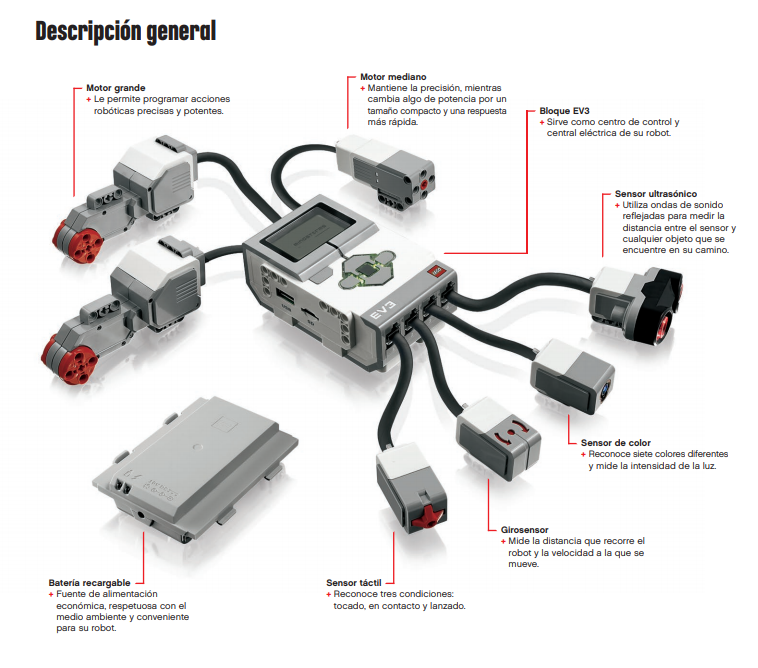
\includegraphics[scale=0.7]{img/partes.png}
    \caption{Conjunto Ev3} \label{fig:partes}
\end{figure}
 Esto quiere decir que las posibilidades a la hora de crear diferentes robots, con diferentes configuraciones de sensores, son prácticamente infinitas. Pero vamos a centrarnos en los casos que mas funcionalidad tienen. El robot que mas versatilidad presenta a la hora de superar ejercicios, es un robot triciclo, con dos ruedas delanteras y una pivotante trasera. Así que este será nuestro modelo para el robot. Y ademas como el \textit{kit de LEGO MINDSTORMS} viene con tres sensores diferentes, crearé tres modelos para integrarlos por separado en la plataforma.
  \begin{figure}[H]
    \centering
    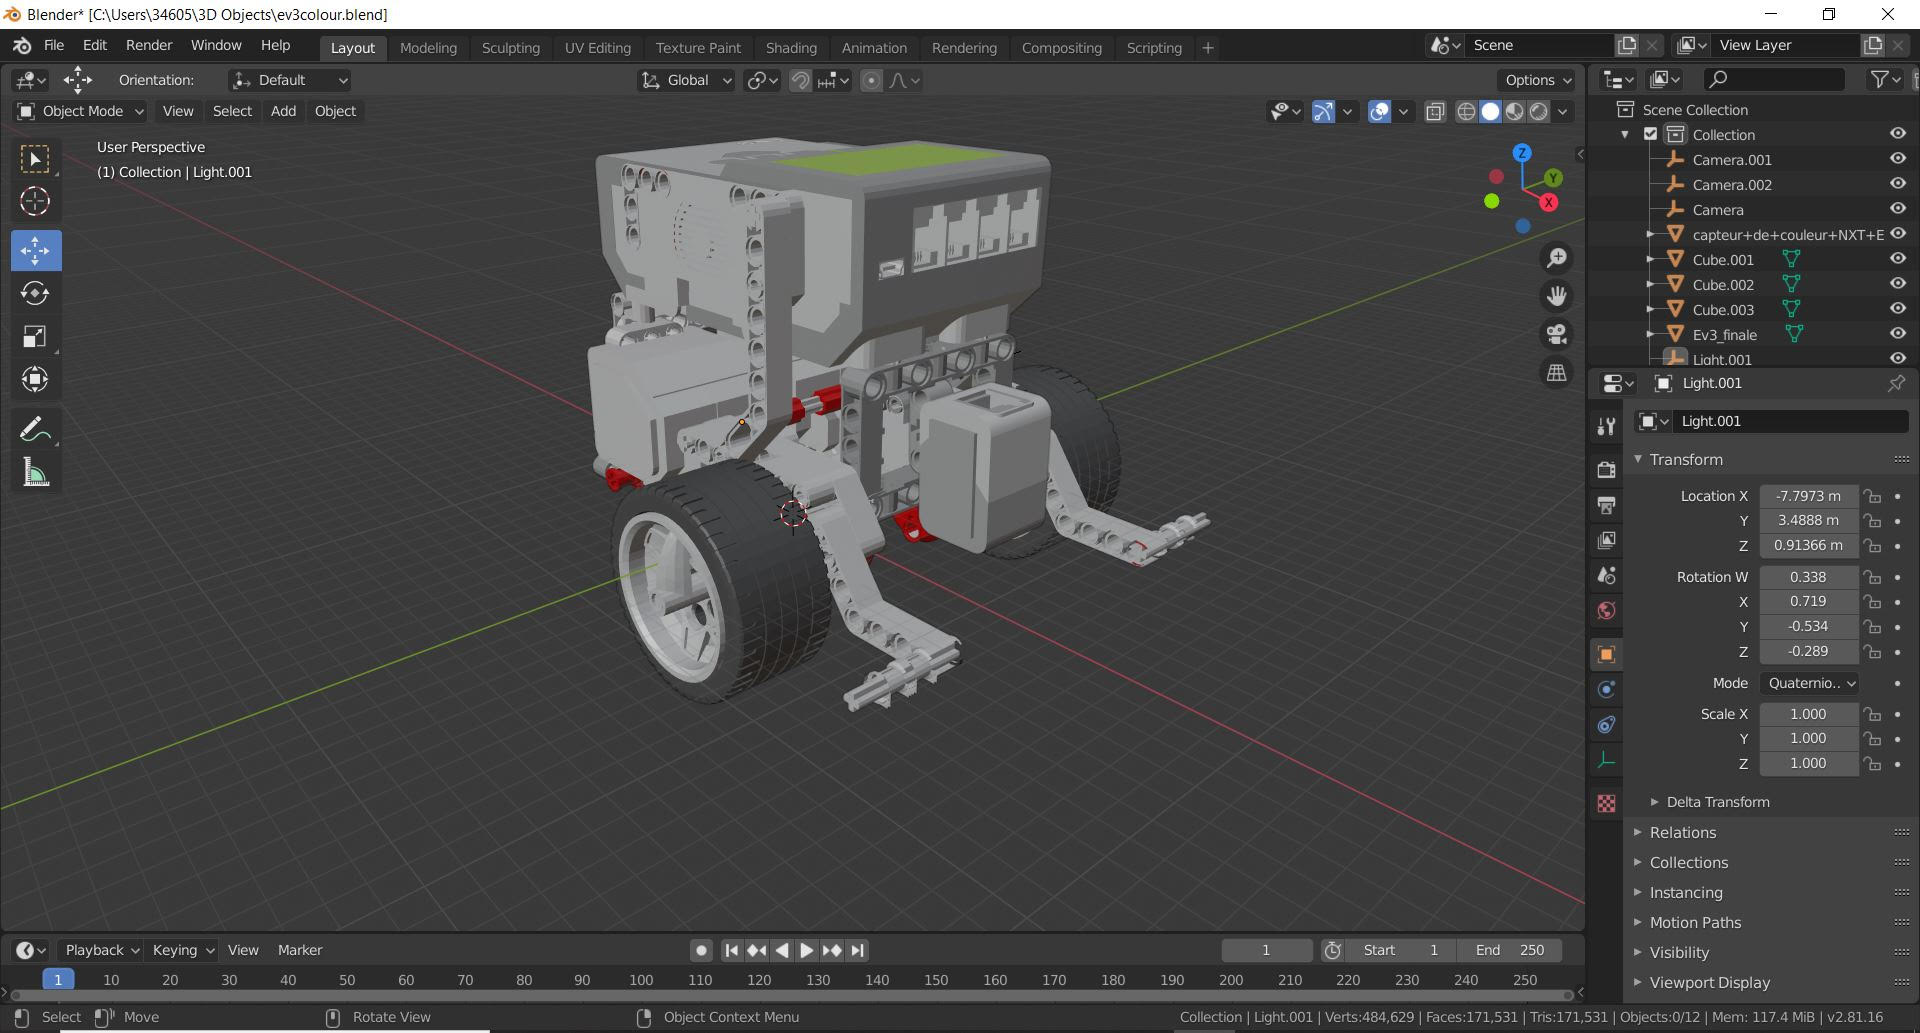
\includegraphics[width=0.7\textwidth]{img/blendercolor.jpg}
    \caption{Robot con sensor de color} \label{fig:color}
\end{figure}
 \begin{figure}[H]
    \centering
    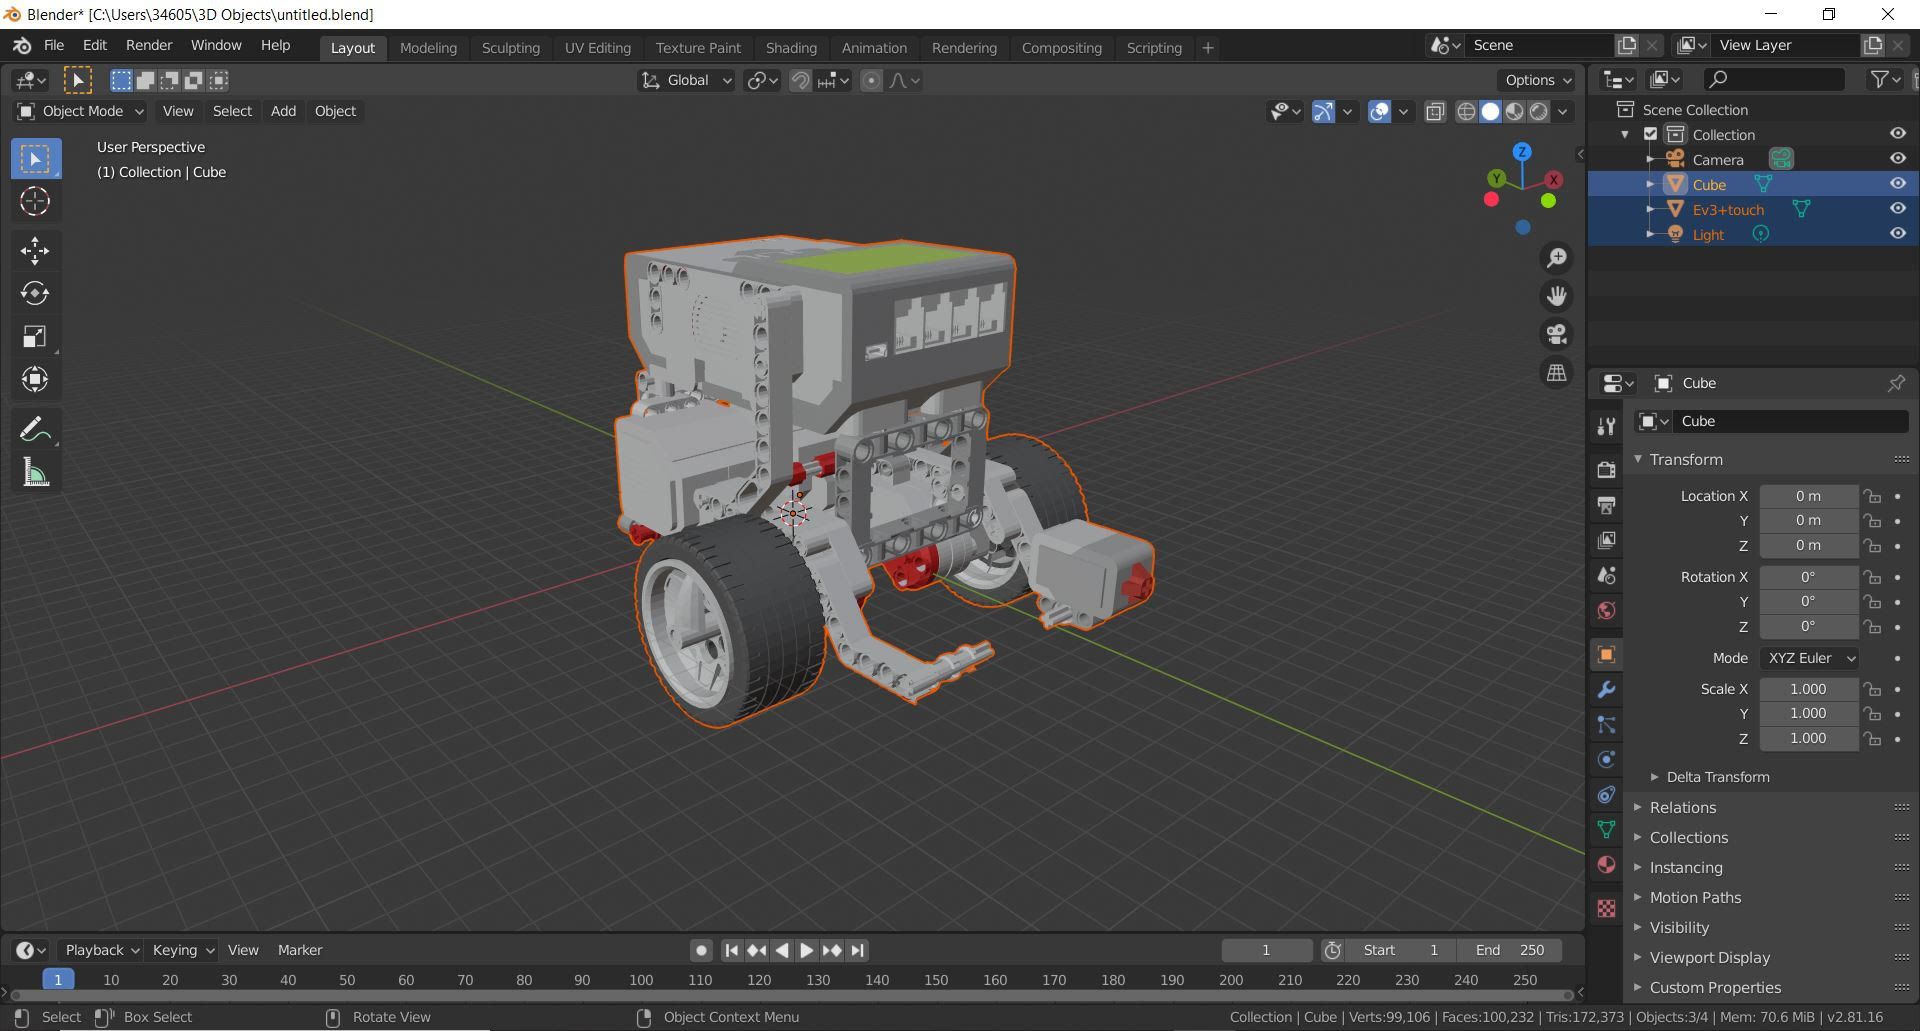
\includegraphics[width=0.7\textwidth]{img/blendertouch.jpg}
    \caption{Robot con sensor tactil} \label{fig:tactil}
\end{figure}
 \begin{figure}[H]
    \centering
    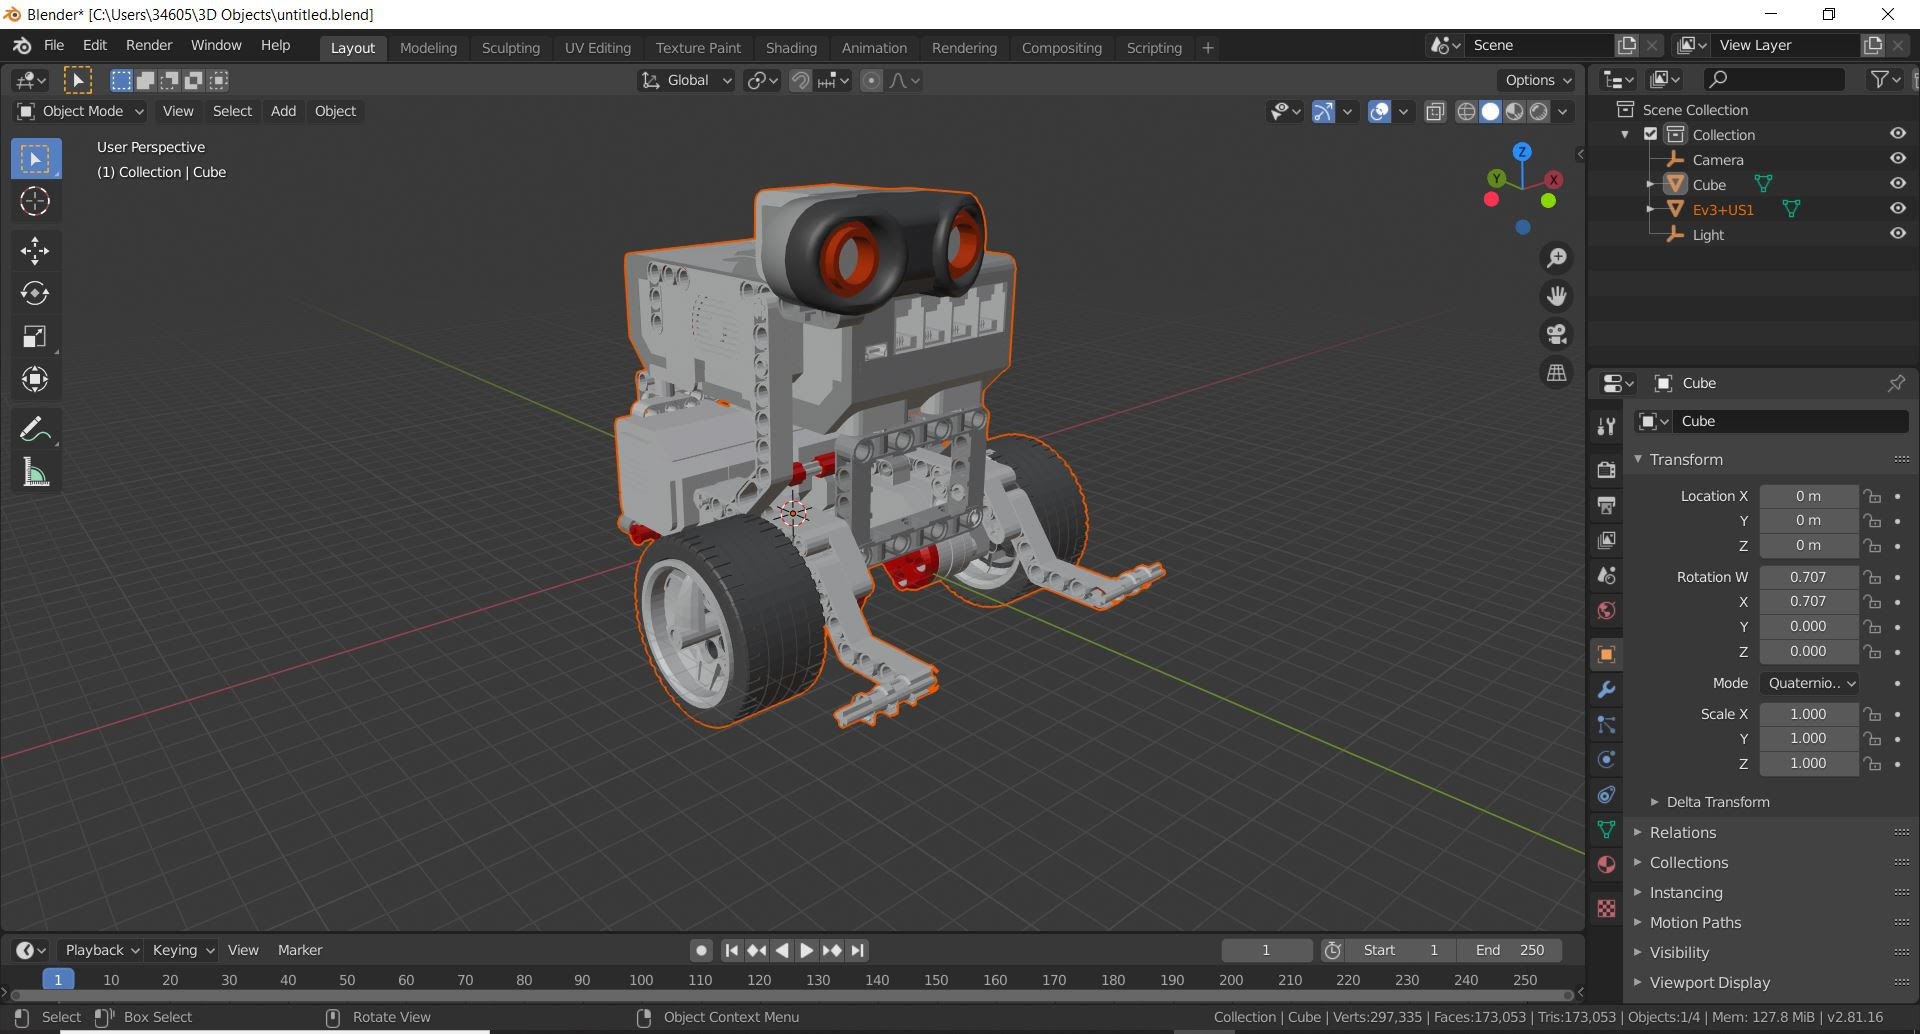
\includegraphics[width=0.7\textwidth]{img/blenderus.jpg}
    \caption{Robot con sensor de ultrasonidos} \label{fig:ultrasonidos}
\end{figure}
Para la tarea del modelaje 3D, he usado el programa de \textit{Blender}. \newline
Ahora que tenemos los tres modelos, voy a dividir el soporte del robot simulado en los diferentes sensores que implementar.
\section{Soporte de sensores}
\label{sec:sensores}

\subsection{Sensor de color}

El primer sensor que vamos a analizar es el sensor de color. El Sensor de color es un sensor digital que puede detectar el color o la intensidad de la luz que ingresa por la pequeña ventana de la cara del sensor. Este sensor puede utilizarse en tres modos diferentes: Modo color, Modo intensidad de la luz reflejada y Modo intensidad de la luz ambiental.\newline
La tasa de muestreo del sensor de color es de 1 kHz.
\begin{wrapfigure}{l}{0.3\linewidth}
    \centering
    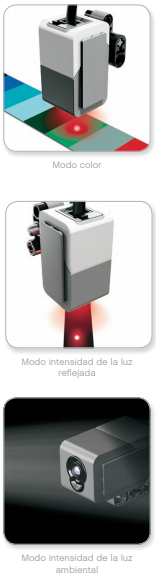
\includegraphics[width=0.6\linewidth]{img/color.png}
    \caption{Sensor color}{{\footnotesize Sensor de color en sus 3 usos}}
    \label{fig:color}
\end{wrapfigure}

\begin{itemize}
\item\textbf{En Modo color}, el Sensor de color reconoce siete colores: negro,
azul, verde, amarillo, rojo, blanco y marrón, además de Sin color.Esta capacidad de diferenciar los colores significa que su robot puede estar programado para clasificar pelotas o bloques de colores, y realizar acciones diferentes con cada color detectado.\newline
Este tipo de acciones, están ya contempladas en la funcionalidad del \textit{HAL API} de \textit{Kibotics}. Aunque en este caso utiliza una camara simulada para comprobar que color esta viendo.\newline
\textit{\textbf{getImage(cameraID)}}: Método que devuelve  \textit{robot}. 
    
    \begin{lstlisting}[language=javascript]
   function getImage(cameraID) {
    /**
     * Returns a screenshot from the robot camera
     */
    if (!cameraID || (this.camerasData.length === 1) || 
    (cameraID > this.camerasData.length - 1)) {
        return this.camerasData[0]['image'];
    } else {
        return this.camerasData[cameraID]['image'];
    }

}
    \end{lstlisting}
\end{itemize}

El \textit{LEGO EV3} no tiene una camara instalada, pero para el robot simulado, es lo mas sencillo de implementar, ya que puede analizar la imagen simulada y sacar el color RGB, para posteriormente dar nombre al color que ve.\newline
\textit{\textbf{getColorRGB()}}: Método que devuelve  \textit{RGB} en tres valores. 
    
    \begin{lstlisting}[language=javascript]
   function getObjectColorRGB(lowval, highval) {
    /**
     * This function filters an object in the scene with a given color, uses OpenCVjs to filter
     * by color and calculates the center of the object.
     *
     * Returns center: CenterX (cx), CenterY (cy) and the area of the object detected in the image.
     */

    if (lowval.length === 3) {
        lowval.push(0);
    }
    if (highval.length === 3) {
        highval.push(255);
    }
    var image = this.getImage();
    var binImg = new cv.Mat();
    var M = cv.Mat.ones(5, 5, cv.CV_8U);
    var anchor = new cv.Point(-1, -1);
    var lowThresh = new cv.Mat(image.rows, image.cols, image.type(), lowval);
    var highThresh = new cv.Mat(image.rows, image.cols, image.type(), highval);
    var contours = new cv.MatVector();
    var hierarchy = new cv.Mat();

    cv.morphologyEx(image, image, cv.MORPH_OPEN, M, anchor, 2,
        cv.BORDER_CONSTANT, cv.morphologyDefaultBorderValue()); // Erosion followed by dilation

    cv.inRange(image, lowThresh, highThresh, binImg);
    cv.findContours(binImg, contours, hierarchy, cv.RETR_CCOMP, cv.CHAIN_APPROX_SIMPLE);
    if (contours.size() > 0) {

        let stored = contours.get(0);
        var objArea = cv.contourArea(stored, false);

        let moments = cv.moments(stored, false);
        var cx = moments.m10 / moments.m00;
        var cy = moments.m01 / moments.m00;

    }
    return {center: [parseInt(cx), parseInt(cy)], area: parseInt(objArea)};
}
    \end{lstlisting}
    
Una vez realizado este paso podemos ponerle un nombre al color, como hace el \textit{LEGO EV3} real.

\begin{itemize}
\item\textbf{En Modo intensidad de la luz reflejada}, el Sensor de color mide la intensidad de la luz que se refleja desde una lámpara emisora de luz color rojo. El sensor utiliza una escala de 0 (muy oscuro) a 100 (muy luminoso). Esto significa que su robot puede estar programado para moverse sobre una superficie blanca hasta detectar una línea negra o para interpretar una tarjeta de identificación con código de color.
Esto en el robot simulado, es diferente, ya que no podemos ver como una magnitud física como es la luz se refleja un objeto, pero este efecto depende del color que se este viendo en la imagen, la luminosidad del color se puede calcular con esta función:

\textit{\textbf{getLightness(valuemin, valuemax)}}: Método que devuelve  \textit{Luminosidad}. 
    
    \begin{lstlisting}[language=javascript]
   function getLightness(valuemin, valuemax) {
    
    let image = this.getObjectColorRGB(valuemin, valuemax);
    let L = ((image.center[0]- image.center[1])/2)*100/255;
    
    /**
     * Returns lightness with a percent
     */
    
    return L.

}
\end{lstlisting}

Esta funcion puede resultar util, para, por ejemplo, poder seguir una linea, cuando haya colores muy similares, o cuando se este utilizando el robot en una mesa o superficie alta, detectar antes, donde esta el borde.

\item\textbf{En Modo intensidad de la luz ambiental}, el Sensor de color mide la intensidad de la luz que ingresa en la ventana desde su entorno, como la luz del sol o el haz de una linterna. El sensor utiliza una escala de 0 (muy oscuro) a 100 (muy luminoso). Esta funcionalidad, no puede ser implementada en la plataforma, ya que no tenemos un foco de luz que se puede analizar, ni tampoco una magnitud dentro del entorno que represente la luz.

\end{itemize}

\subsection{Sensor de ultrasonido}

El Sensor ultrasónico es un sensor digital que puede medir la distancia a un objeto que se encuentra frente a él. Para hacerlo, envía ondas de sonido de alta frecuencia y mide cuánto tarda el sonido en reflejarse de vuelta al sensor. La frecuencia de sonido es demasiado alta para el oído humano.
La distancia a un objeto puede medirse en pulgadas o centímetros.\newline
\begin{wrapfigure}{r}{0.5\linewidth}
    \centering
    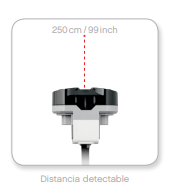
\includegraphics[width=0.5\linewidth]{img/ultrasonidos.png}
    \caption{Sensor de ultrasonidos}
    \label{fig:ultrasonido}
\end{wrapfigure}
Esto le permite programar su robot para que se detenga a una distancia determinada de una pared. Al utilizar unidades en centímetros, la distancia detectable es entre 3 y 250 centímetros (con una exactitud de +/- 1 centímetro). Al utilizar unidades en pulgadas, la distancia detectable es entre 1 y 99 pulgadas (con una exactitud de +/- 0,394 pulgadas). Un valor de
255 centímetros o 100 pulgadas significa que el sensor no puede
detectar ningún objeto frente a él.\newline
En \textit{Kibotics} la implementación que hay para las distancias es  usar un \textit{RayCaster}. Que es equivalente a poner láseres apuntando hacia todas direcciones por delante del robot de esta forma:

\begin{figure}[H]
    \centering
    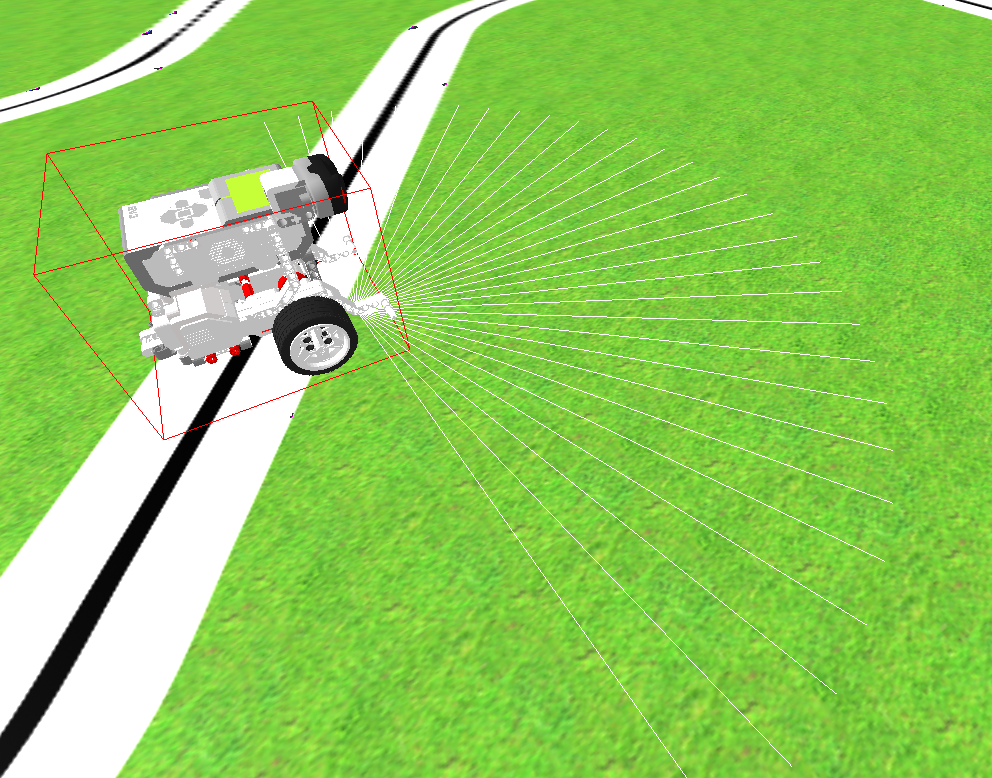
\includegraphics[width=0.7\textwidth]{img/pruebaUS.png}
    \caption{Raycaster} \label{fig:raycaster}
\end{figure}

Lo cual devuelve un \textit{array} de valores con las distancias a las que "rebota" cada láser. Esto tratándose de un sensor ultrasonidos que solo devuelve un único valor con el obstáculo mas cercano, es un poco irreal. Por lo que creare la función \textit{getDistance} que devuelve el valor mas cercano de todos los que hay en el \textit{array} de \textit{RayCaster} 

\textit{\textbf{Funciones que calculan la distancia}}: Método que devuelve  un unico valor con la distancia mas corta. 

 \begin{lstlisting}[language=javascript]
function getDistance() {
    /**
     * This function returns the distance for the raycaster in the center of the arc of rays.
     */
    var distances = this.getDistances();

    if (distances[13] !== 10 || distances[14] !== 10 || distances[15] !== 10 || distances[16] !== 10 || distances[17] !== 10) {
        let distance0 = 100;
        let distance1 = 100;
        let distance2 = 100;
        let distance3 = 100;
        let distance4 = 100;
        if (distances[13] !== 10) {
            distance0 = distances[13];
        }
        if (distances[14] !== 10) {
            distance1 = distances[14];
        }
        if (distances[15] !== 10) {
            distance2 = distances[15];
        }
        if (distances[16] !== 10) {
            distance3 = distances[16];
        }
        if (distances[17] !== 10) {
            distance4 = distances[17];
        }
        let min_distances = [distance0, distance1, distance2, distance3, distance4];
        Array.min = function (array) {
            return Math.min.apply(Math, array);
        };
        return Array.min(min_distances);
    } else {
        return 10;
    }
}

function getDistances() {
    /**
     * This function returns an array with all the distances detected by the rays.
     */
    var distances = [];
    for (var i = 0; i <= 31; i++) {
        distances.push(10);
    }
    var groups = ["center", "right", "left"];
    for (i = 0; i < groups.length; i++) {
        this.distanceArray[groups[i]].forEach((obj) => {
            if (typeof obj.d != "undefined") {
                distances[obj.id] = obj.d;
            }
        });
    }
    return distances;
}
\end{lstlisting}

\subsection{Sensor de contacto}

El Sensor táctil es un sensor analógico que puede detectar el momento en el que se presiona y se lanza el botón rojo del sensor. Esto significa que el Sensor táctil puede programarse para actuar según tres condiciones: presionado, lanzado o en contacto (tanto presionado como lanzado). Con la información del Sensor táctil, se puede programar un robot para ver el mundo como lo haría una persona no vidente, es decir, extendiendo un brazo y respondiendo cuando toca algo (presionado).
\begin{wrapfigure}{r}{0.5\linewidth}
    \centering
    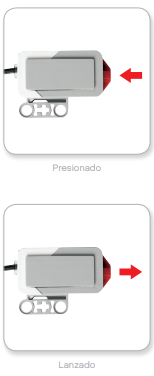
\includegraphics[width=0.5\linewidth]{img/tactil.png}
    \caption{Sensor tactil}
    \label{fig:tactil}
\end{wrapfigure}
Puede construir un robot con un Sensor táctil presionado contra la superficie. Luego, puede programar el robot para que responda (se detenga) cuando esté a punto de pasar el borde de la mesa (cuando el sensor se lanza). Un robot de pelea puede programarse para continuar empujando hacia adelante en dirección a su oponente hasta que este se retire. Ese par de acciones, presionado y lanzado, constituyen el estado En contacto.

En la plataforma, no había ninguna función similar que implementara un sensor de contacto. Así que, creare un par de funciones, que aprovechándose del \textit{array} de distancias, cogeré la distancia central y cuando sea mínima, daré por hecho que el robot esta tocando la superficie

   \begin{lstlisting}[language=javascript]
     getCenterDistance(){
      
      if (this.distanceArray["center"][0] != null) {
          return this.distanceArray["center"][0].d;
      } else {
          return 10;
      }
    }
    isTouching() {
        return (this.getCenterDistance()<3);
    }
\end{lstlisting}

Esta función al ser totalmente nueva, habrá que añadirla en el \textit{HAL API} y tendrá que tener su equivalente en \textit{Python} y en \textit{Blockly}, que mostrare en la siguiente parte con la implementación de este sensor en un ejercicio.

\subsection{Girosensor}
El Girosensor es un sensor digital que detecta el movimiento de rotación en un eje simple. Si rota el Girosensor en la dirección que indican las flechas que se encuentran en la caja del sensor, este puede detectar la razón de rotación en grados por segundo. (El sensor puede medir una razón de giro máxima de 440 grados por segundo.) Entonces, puede utilizar la razón de rotación para detectar, por ejemplo, si gira una parte del robot o si el robot se cae.

\begin{wrapfigure}{l}{0.5\linewidth}
    \centering
    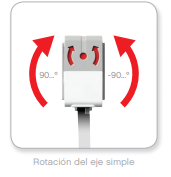
\includegraphics[width=0.5\linewidth]{img/gyrosensor.png}
    \caption{girosensor}
    \label{fig:girosensor}
\end{wrapfigure}

Además, el Girosensor registra el ángulo de rotación total en grados. Puede utilizar este ángulo de rotación para detectar, por ejemplo,cuánto ha girado su robot. Esta función le permite programar giros (sobre el eje que está midiendo el Girosensor) con una exactitud de +/- 3 grados en un giro de 90 grados.

Este sensor no requiere una implementacion dentro de la plataforma ya que, el único uso que puede darse dentro de la plataforma, es medir un giro de unos grados que pasas como argumentos. Y eso ya esta implementado en el \textit{HAL API}. El otro uso real que se le puede dar a este sensor es para que un robot mantenga el equilibrio dinámico, mientras se mueve. Pero en \textit{Kibotics}, no tienen un centro de gravedad en el mantenerse.

  
\section{Nuevos ejercicios}
\label{sec:ejercicios}

Se han añadido ejercicios para comprobar la funcionalidad de cada uno de los sensores anteriormente explicados 

\subsection{Sigue-líneas}
    Este ejercicio consiste en seguir una línea negra en el suelo sobre fondo blanco haciendo uso de la cámara del \textit{robot}, que recoge las imágenes y las filtra para poder seguirla.
    
    
    \begin{figure}[H]
    \centering
    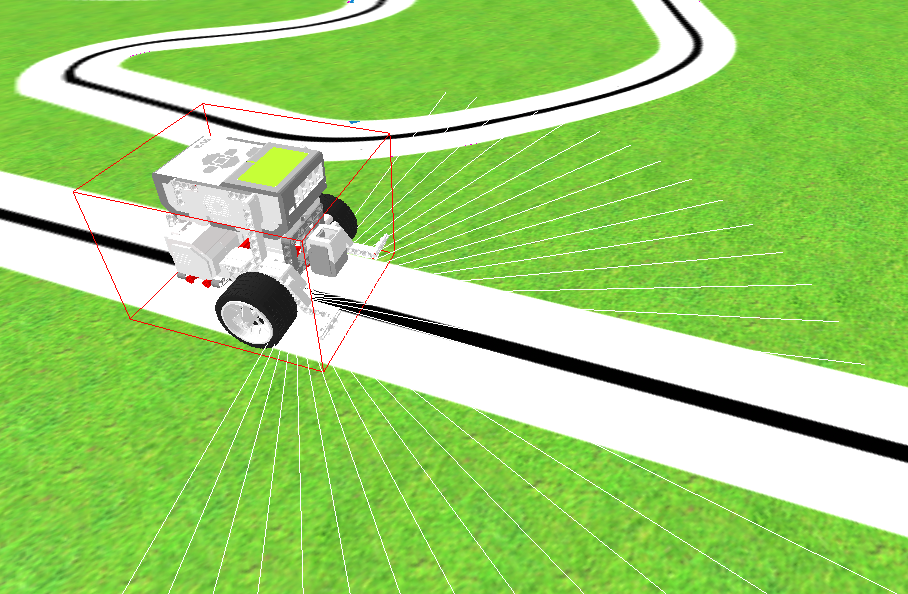
\includegraphics[scale=0.4]{img/siguelineas.png}
    \caption{Escenario para el ejercicio \textit{LEGO EV3} sigue-líneas} \label{fig:siguelinea}
    \end{figure}
    
        \begin{figure}[H]
    \centering
    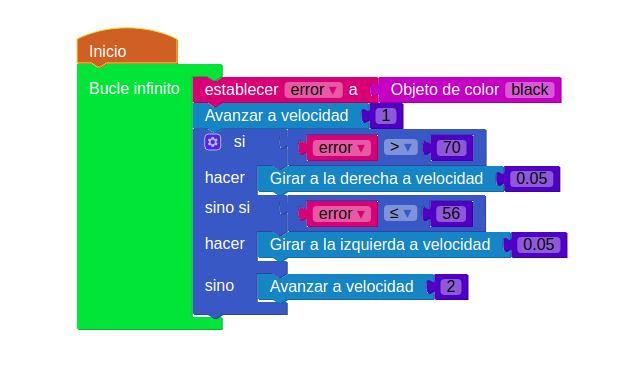
\includegraphics[scale=0.5]{img/solucion.png}
    \caption{Solución en \textit{Scratch} para el ejercicio sigue-líneas} 
    \label{fig:solucion}
    \end{figure}
    
En la solución se establece un error con el color negro, de modo que dependiendo del lado por el que me pase, corrijo girando hacia al lado contrario
    
    
\subsection{Choca-gira}
\label{subsec:chocagira}
En este ejercicio hay programar al \textit{robot} para que avance recto mientras no haya obstáculos haciendo uso del sensor de ultra-sonidos. Si encuentra un obstáculo, tiene que detenerse, retroceder un poco, girar a la derecha y seguir adelante.


    \begin{figure}[H]
    \centering
    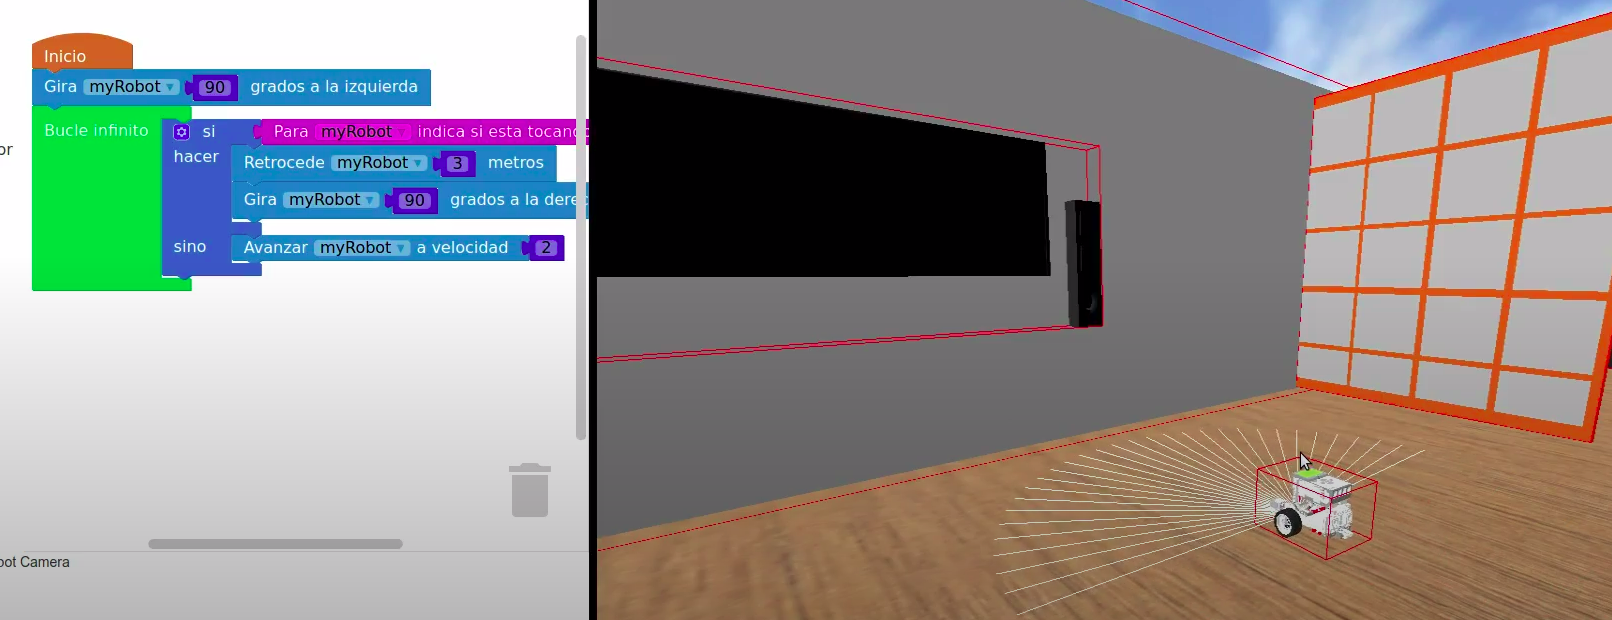
\includegraphics[scale=0.25]{img/chocagira.png}
    \caption{Solución en \textit{Scratch} para el ejercicio choca-gira} 
    \label{fig:chocagira}
    \end{figure}
    
    En esta solución\footnote{\url{https://youtu.be/figTbXKEXD4}} se prueba el bloque anteriormente mencionada que equivale a la funcion \textit{IsTouching} en el lenguaje \textit{Scratch}.
    
\subsection{Atraviesa-bosque}
\label{subsec:atraviesabosque}
Ejercicio basado en atravesar un pasillo con diversos objetos que hay que esquivar. El sensor necesario es el infrarrojos para detectar en que posición se encuentra el siguiente obstáculo. Este ejercicio solo se puede hacer simuladamente, ya que el \textit{LEGO EV3} con el sensor ultrasonido no puede saber en que posición se encuentra el obstáculo, solo la distancia. Aún así, este ejercicio tiene un gran interés educativo, por lo que he decidido añadirlo, y ademas crear una nueva función para que sea mas sencillo e intuitivo de completar para el estudiante.

\textit{\textbf{GetMinorDistance}}: Método que devuelve en que dirección se encuentra el obstáculo más cercano. 

 \begin{lstlisting}[language=javascript]
 getMinorDistance() {
      /*
        This function returns the minor distance of an array with all distances
      */

      var distances = []
      let ray = 32;
      let distance=5;
      for (var i = 0; i <= 31; i++) {
          distances.push(10);
      }
      var groups = ["center", "right", "left"];
      for (var i = 0; i < groups.length; i++) {
          this.distanceArray[groups[i]].forEach((obj) => {
              if (typeof obj.d != "undefined") {
                  distances[obj.id] = obj.d;
              }
          });
      }
      for (var i=0; i<distances.length; i++){
        if (distances[i]<distance){
          distance=distance[i]
          ray=i;
        }
      }
      if (ray > 15 && ray < 32) {
          return groups[1];

      }else if(ray == 15){
          return groups[0];

      } else if (ray < 15) {
          return groups[2];

      }else {
          return "unhindered";
      }
    }
 
 
 \end{lstlisting}

Con esta función se puede resolver el ejercicio con un simple bucle que distingue entre las tres opciones que devuelve.

    \begin{figure}[H]
    \centering
    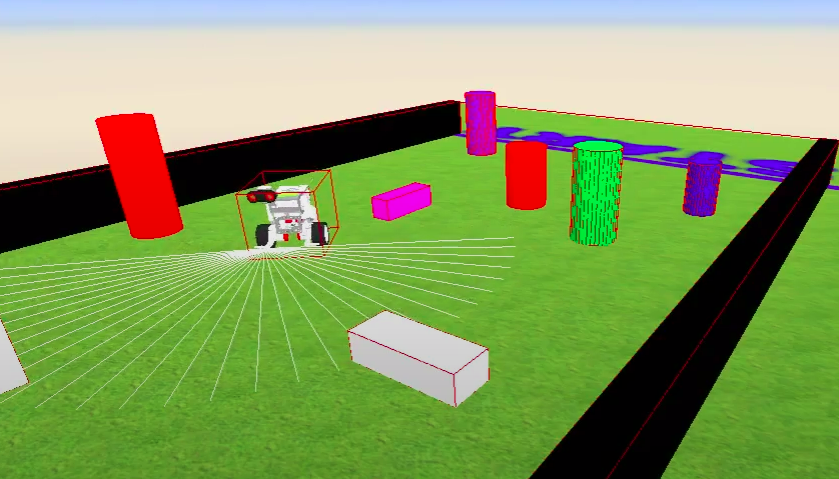
\includegraphics[scale=0.45]{img/forest.png}
    \caption{Escenario para el ejercicio atraviesa bosque} 
    \label{fig:atraviesaBosque}
    \end{figure}

    \begin{figure}[H]
    \centering
    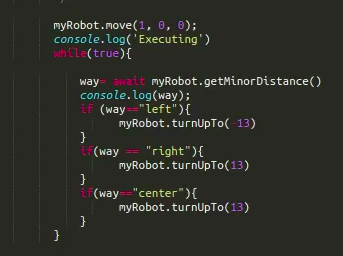
\includegraphics[scale=0.6]{img/solucionforest.png}
    \caption{Solución en \textit{JavaScript} para el ejercicio atraviesa bosque} 
    \label{fig:solucionforest}
    \end{figure}
    
    En esta solución\footnote{\url{https://youtu.be/ZSYWMSSRkS8}} se obtienen todos los valores que devuelve el sensor de ultra-sonidos y, según donde detecte el obstáculo, gira en un sentido u otro.


